\documentclass[10pt]{beamer}
\usetheme{Madrid}
\usecolortheme{default}
\setbeamertemplate{footline}{} % Disable footer
\setbeamertemplate{navigation symbols}{} % Remove navigation icons

\usepackage[utf8]{inputenc}
\usepackage{graphicx}
\usepackage{amsmath}
\usepackage{amsfonts}
\usepackage{amssymb}
\usepackage{booktabs}
\usepackage{array}
\usepackage{listings} % For code snippets

% --- Project Details ---
\title{Virtual Physical Therapist: AI-Powered Movement Assessment and Exercise Guidance}
\subtitle{S7 B.Tech AIML Project - Phase 1 Review}
\author{
\textbf{Abhiram P S (VAS22AIM004)\\
 Govind P Vinod (VAS22AIM024)\\
 Sahna Saleeph (VAS22AIM049)\\
 Shahzad Bin Mohamed (VAS22AIM050)\\ }}
\institute{
    \textbf{Guided by:}\\
    Ms Linsa V.U, Assistant Professor, DoAIML\\
    \\

    Vidya Academy of Science and Technology\\
    Department of Artificial Intelligence and Machine Learning\\
    6th October 2025
}
\date{}

% Add college logo
\logo{
\includegraphics[height=0.8cm]{college_logo.jpg}} % Make sure you upload a 'college_logo.jpg' file

\begin{document}

% --- Title Slide ---
\begin{frame}
\titlepage
\end{frame}

% --- Vision and Mission ---
\begin{frame}{Vision and Mission}
\begin{center}
    
\includegraphics[width=4cm]{college_logo.jpg} % Replace with your actual image file name

    \vspace{0.8cm}

    \textbf{College Vision:} \\
    Progress Through Education

    \vspace{0.8cm}

    \textbf{College Mission:} \\
    To seek, strive for and scale greater heights of quality education
\end{center}
\end{frame}

% --- Department Vision and Mission ---
\begin{frame}{Dept Vision and Mission}
\begin{center}
    
\includegraphics[width=3cm]{college_logo.jpg} % Replace with your department logo file

    \vspace{0.2cm}

    \textbf{Dept Vision:} \\
    To evolve as a center of excellence for higher education in the field of Artificial Intelligence and Machine Learning

    \vspace{0.4cm}

    \textbf{Dept Mission:}
\end{center}

\vspace{0.4cm}

\textbf{M1:} To equip the graduates with the latest technologies in the field of Artificial Intelligence and Machine Learning.

\vspace{0.3cm}

\textbf{M2:} To imbibe new knowledge by collaborating with industry and research organizations to mould competent technocrats and entrepreneurs.

\vspace{0.3cm}

\textbf{M3:} To instill societal and ethical responsibilities in all professional activities.
\end{frame}


% --- Contents ---
\begin{frame}{Contents}
    \begin{enumerate}
        \item Introduction
        \item Aim
        \item Objectives
        \item Methodology
        \item System Architecture
        \item Implementation Details
        \item Results \& Live Demo
        \item Conclusion
        \item References
    \end{enumerate}
\end{frame}


% --- Introduction ---
\begin{frame}{Introduction}
    \frametitle{Introduction: The Problem}
    \begin{itemize}
        \item Access to professional physical therapy is often expensive and inconvenient.\vspace{0.5em}
        \item Individuals exercising alone frequently use incorrect form, leading to a high risk of injury.\vspace{0.5em}
        \item Traditional fitness apps provide instructions but lack real-time, personalized feedback on a user's actual movements.\vspace{0.5em}
        \item There is a need for an accessible, low-cost system that can analyze and correct exercise form in real-time using only a standard webcam.
    \end{itemize}
\end{frame}


% --- Aim ---
\begin{frame}{Aim}
    \frametitle{Project Aim}
    To design and develop an intelligent virtual physical therapist that leverages computer vision to provide real-time movement assessment, accurate repetition counting, and actionable feedback on exercise form, accessible through a standard camera.
\end{frame}


% --- Objectives ---
\begin{frame}{Objectives}
    \frametitle{Project Objectives}
    \begin{itemize}
        \item Build a real-time human pose estimation module using a standard webcam to track key body joints.\vspace{0.5em}
        \item Develop algorithms to calculate critical joint angles for specific exercises (e.g., squats, bicep curls).\vspace{0.5em}
        \item Implement a robust, state-based repetition counting system.\vspace{0.5em}
        \item Create a real-time accuracy scoring system by comparing the user's form against a calibrated reference motion.\vspace{0.5em}
        \item Provide intuitive visual feedback via a skeleton overlay and a dynamic accuracy bar.\vspace{0.5em}
        \item Design a visual calibration tool to allow new exercises to be added to the system easily.
    \end{itemize}
\end{frame}


% --- Methodology ---
\begin{frame}{Methodology: Phase 1}
    \frametitle{Methodology: Real-Time Pose Estimation}
    \begin{itemize}
        \item \textbf{Primary Technology:} MediaPipe Pose.\vspace{0.5em}
        \item \textbf{Function:} Provides real-time detection of 33 key body landmarks (joints) from each video frame.\vspace{0.5em}
        \item \textbf{Process:}
        \begin{itemize}
            \item The system captures a video feed using OpenCV.
            \item Each frame is passed to the MediaPipe Pose model.
            \item The model returns the 2D coordinates (\textit{x, y}) for each landmark.
        \end{itemize}\vspace{0.5em}
        \item \textbf{Advantage:} Forms the foundation for all subsequent analysis by providing the raw data to understand posture and movement. It is lightweight and runs efficiently on standard CPUs.
    \end{itemize}
\end{frame}

\begin{frame}{Methodology: Phase 2}
    \frametitle{Methodology: Exercise Logic \& Feedback}
    \begin{itemize}
        \item \textbf{Angle Calculation:} A custom Python function uses vector mathematics to calculate the 2D angle between three connected joints (e.g., Shoulder-Elbow-Wrist).\vspace{0.5em}
        \item \textbf{Repetition Counting:} A state machine logic tracks whether the user is in the "up" or "down" phase of an exercise based on angle thresholds. A rep is counted only on a full "down" to "up" state transition.\vspace{0.5em}
        \item \textbf{Accuracy Score:} The user's live angles are compared against a pre-recorded "perfect rep". The system intelligently syncs the user's movement phase with the reference data to calculate a weighted average of the angular differences, producing an intuitive accuracy score.
    \end{itemize}
\end{frame}

\begin{frame}{Methodology: Phase 3}
    \frametitle{Methodology: System Usability \& Calibration}
    \begin{itemize}
        \item \textbf{Visual Calibration Tool:} A standalone GUI application (\texttt{visual\_calibrator.py}) built with PyQt5.\vspace{0.5em}
        \item \textbf{Functionality:} Allows a non-technical user to define a new exercise by clicking on a skeleton diagram to select joints, name the angle, and assign an accuracy weight.\vspace{0.5em}
        \item \textbf{Reference Motion Generation:} The calibrator processes a sample video of the new exercise, extracts the landmark and angle data for every frame, and saves it as a structured JSON file in the \texttt{reference\_data/} folder. This file becomes the ground truth for the main application.
    \end{itemize}
\end{frame}


% --- System Architecture ---
\begin{frame}{System Architecture}
    \frametitle{System Architecture}
    \begin{figure}
        \centering
        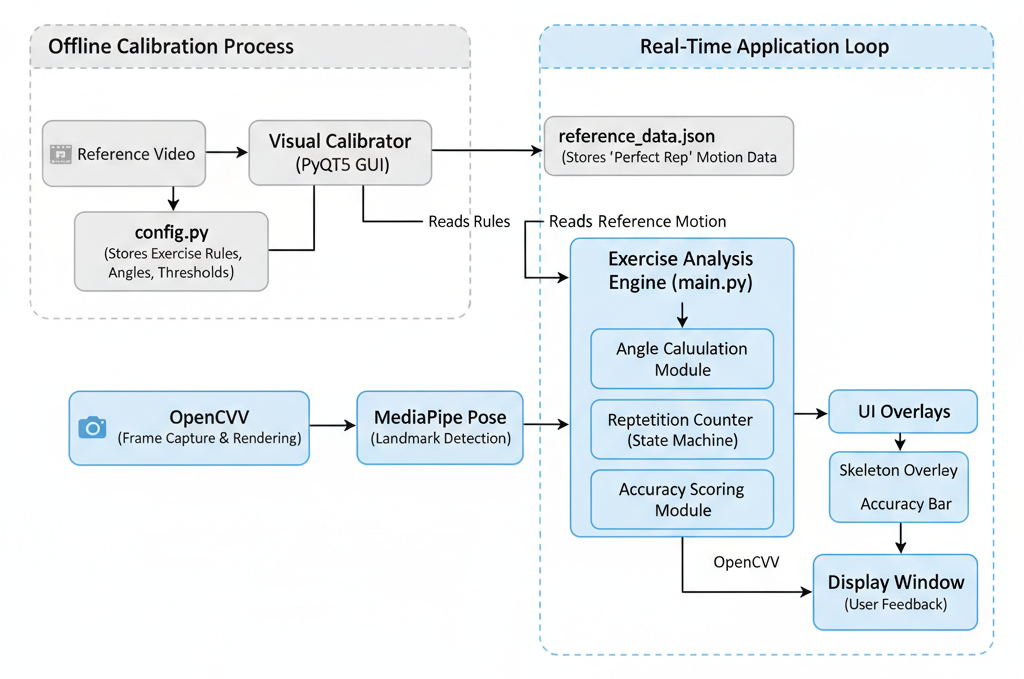
\includegraphics[width=0.9\textwidth]{system_architecture_diagram.png} 
        \caption{High-level data flow of the Virtual PT system.}
    \end{figure}
\end{frame}




% --- Results & Demo ---
\begin{frame}{Results \& Live Demo}
    \frametitle{Results and Application Demo}
    \begin{itemize}
        \item The application successfully runs in real-time, achieving the primary objectives.\vspace{0.5em}
        \item \textbf{Live Pose Tracking:} A skeleton overlay accurately tracks the user's movements.\vspace{0.5em}
        \item \textbf{Repetition Counter:} The UI correctly increments after each complete repetition.\vspace{0.5em}
        \item \textbf{Accuracy Feedback:} The score and color-coded bar update dynamically, providing instant feedback on form quality.\vspace{0.5em}
        \item \textbf{Multi-Exercise Capability:} The system can track different calibrated exercises via command-line arguments.
    \end{itemize}
\end{frame}
\begin{frame}{Results \& Live Demo (Cont.)}
    \begin{figure}
        \centering
        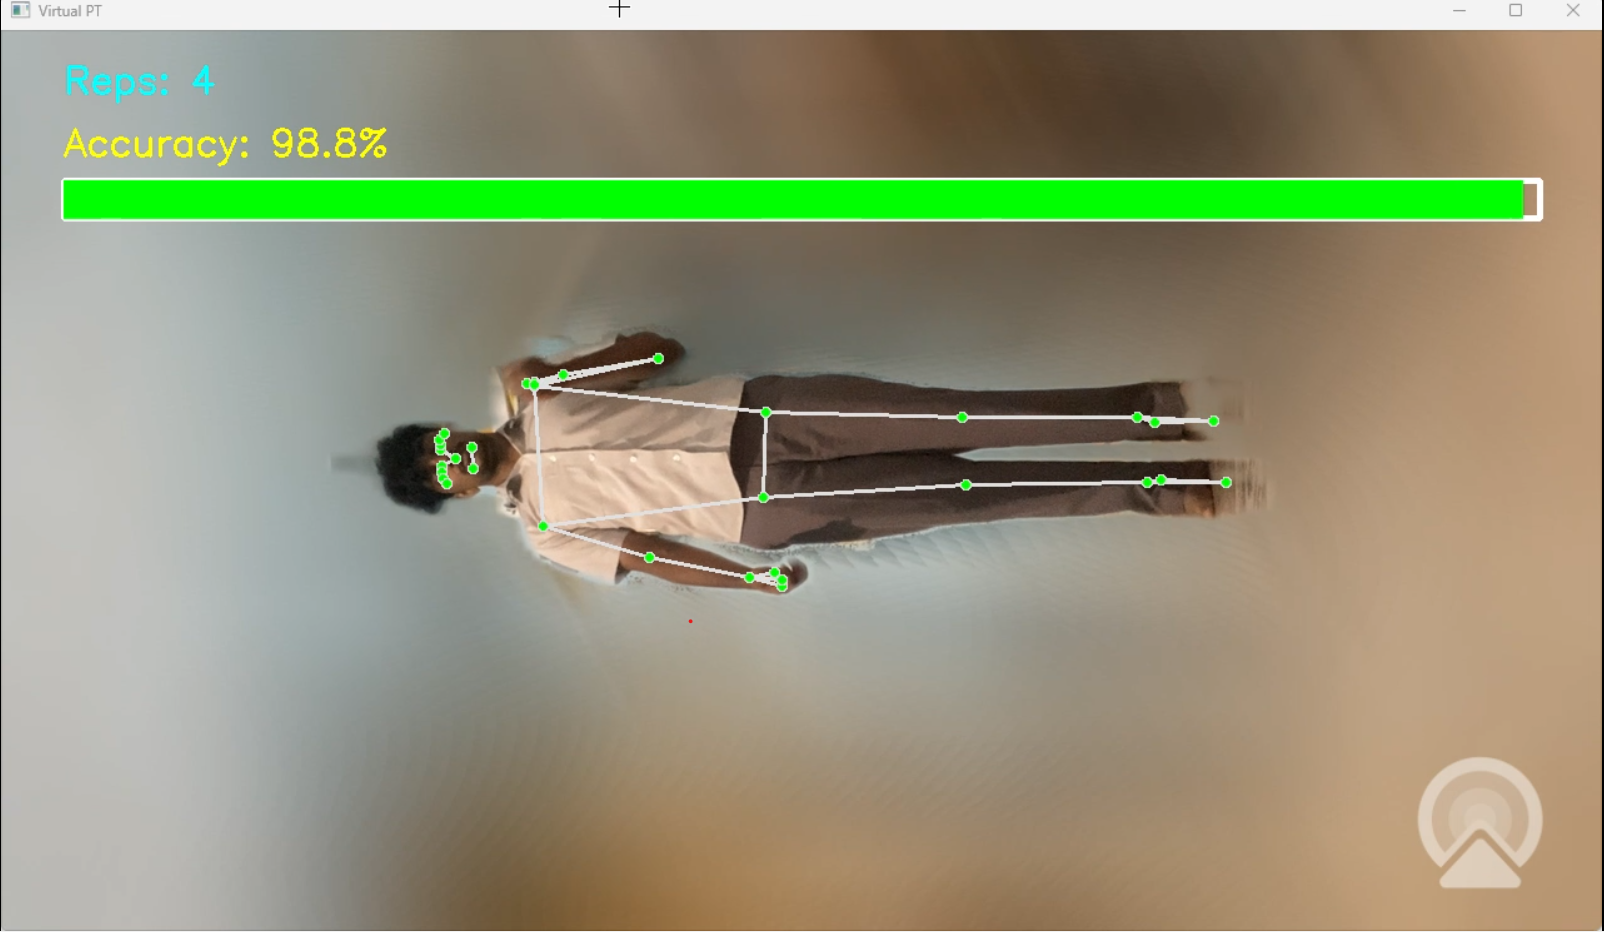
\includegraphics[width=0.4\textwidth]{app.png} 
        \caption{In-App Detection.}
    \end{figure}
        \begin{figure}
        \centering
        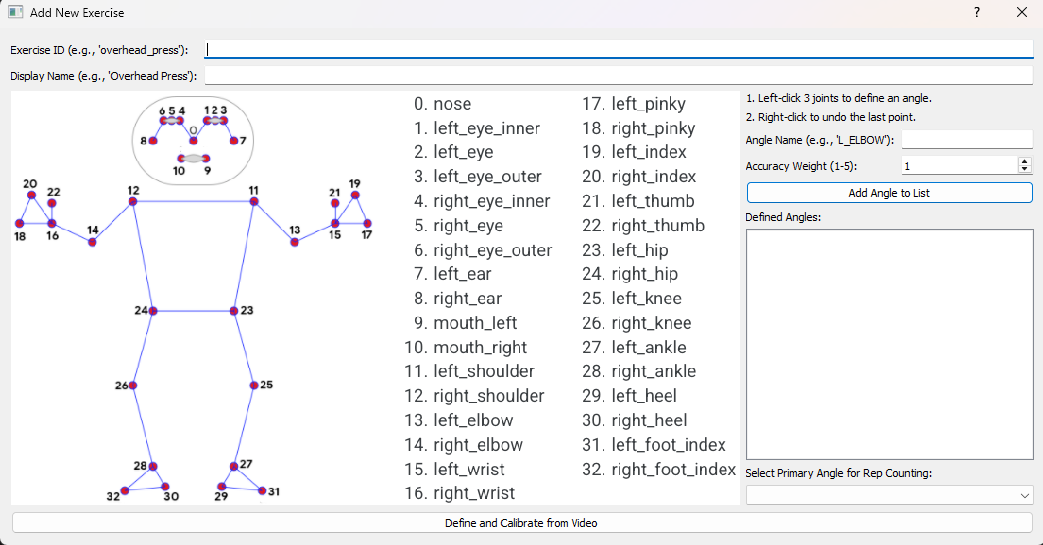
\includegraphics[width=0.4\textwidth]{app2.png} 
        \caption{Easy to use exercise adding system.}
    \end{figure}

\end{frame}


% --- Conclusion ---
\begin{frame}{Conclusion}
    \frametitle{Conclusion and Future Work}
    \begin{itemize}
        \item This project successfully demonstrates a viable framework for an AI-powered Virtual PT using accessible hardware.\vspace{0.5em}
        \item The system provides valuable, real-time feedback on exercise form, helping to increase effectiveness and reduce injury risk.\vspace{0.5em}
        \item The modular design, featuring a unique visual calibration tool, ensures the system is easily extensible.\vspace{0.5em}
        \item \textbf{Future Work:}
        \begin{itemize}
            \item Implement more complex form-correction rules.
            \item Add user profiles to track progress over time.
            \item Develop a more comprehensive GUI for exercise selection.
        \end{itemize}
    \end{itemize}
\end{frame}


% --- References ---
\section{References}
\begin{frame}{References}
\footnotesize
\begin{enumerate}
\item Tharatipyakul, A., Srikaewsiew, T., and Pongnumkul, S.; Deep learning-based human body pose estimation in rehabilitation; Heliyon, 2024. DOI: 10.1016/j.heliyon.2024.e37205

\item Roggio, F., Musumeci, G., and Trovato, B.; A comprehensive analysis of machine learning pose estimation models; Heliyon, 2024. DOI: 10.1016/j.heliyon.2024.e39977

\item Yu, J. and Zhu, D.; Pose estimation for health data analysis: advancing AI in neuroscience and rehabilitation; Frontiers in Neurology, 2025. DOI: 10.3389/fneur.2025.1596408

\item Alshami, A., Nashwan, A., AlDardour, A., and Qusini, A.; Artificial Intelligence in rehabilitation: A narrative review; Rehabilitacion, 2025.
\end{enumerate}
\end{frame}

\begin{frame}{References (Contd.)}
\footnotesize
\begin{enumerate}
\setcounter{enumi}{4}
\item MohammadNamdar, M., Wilson, M.L., Murtonen, K.P., Aartolahti, E., Oduor, M., and Korniloff, K.; How AI-Based Digital Rehabilitation Improves End-User Adherence; JMIR Rehabilitation and Assistive Technologies, 2025.

\item Khalid, U.B., Naeem, M., Stasolla, F., Syed, M.H., Abbas, M., and Coronato, A.; Impact of AI-Powered Solutions in Rehabilitation Process; PMC, 2024.

\item Attoh-Mensah, E., Boujut, A., Desmons, M., and Perrochon, A.; Artificial Intelligence in Personalized Rehabilitation; Frontiers in Digital Health, 2025.

\item Azizan, A.; Global Insights: A Bibliometric Analysis of AI Applications in Rehabilitation; Research and Reviews in Orthopaedics, 2024.
\end{enumerate}
\end{frame}



\end{document}